\documentclass[a4paper]{article}
\usepackage[utf8]{inputenc}
\usepackage{multicol}
\usepackage{multirow}
\usepackage{amsmath}
\usepackage{karnaugh-map}
\usepackage{graphicx}

\title{CSE306 \\
4-bit ALU Simulation}
\author{
  Jawad Ul Kabir\\
  \texttt{1705062}
  \and
  Md. Mahfuzur Rahman Rifat\\
  \texttt{1705063}
  \and
  Taseen Mubassira\\
  \texttt{1705065}
  \and
  Ataf Fazledin Ahamed\\
  \texttt{1705066}
  \and
  Nishat Farhana Purbasha\\
  \texttt{1705067}
}
\date{31 March, 2021}




\begin{document}

\maketitle
\thispagestyle{empty}

\newpage
\clearpage
\pagenumbering{arabic}

\section{Introduction}
An arithmetic logic unit (abbr. ALU) is a multi-operation, combinational-logic digital function- capable of performing a set of basic arithmetic operations and a set of logical operations. The ALU has a set of selection lines which enables a user to select a particular operation in the unit. The selection lines are decoded within the ALU so that $k$ selection variables can specify up to 2$^k$ distinct operations.

\section{Problem Specification with Assigned Instructions}
Design a 4-bit ALU with three selection bits cs0, cs1 and cs2 for performing the following operations:
\newline

% \begin{center}

\begin{table}[ht]
\centering    
\begin{tabular}{|c|c|c|c|}
    \hline
    \multirow{2}{*}{\textbf{cs2}} & \multirow{2}{*}{\textbf{cs1}} & \textbf{cin} & \multirow{2}{*}{\textbf{Functions}}\\
    & & \textbf{cs0} & \\
    \hline
    0 & 0 & 0 & Decrement A \\
    \hline
    0 & 0 & 1 & Transfer A \\
    \hline
    0 & 1 & \times & OR \\
    \hline
    1 & 0 & 0 & Subtract with Borrow \\
    \hline
    1 & 0 & 1 & Subtract \\
    \hline
    1 & 1 & \times & Complement A \\
    \hline
\end{tabular}
\end{table} 

% \end{center}

\section{Truth Table and K-maps}
Truth table for the functions:
\newline

\begin{table}[ht]
\centering
\begin{tabular}{|c|c|c|c|c|c|c|}
    \hline
    \textbf{cs2} & \textbf{cs1} & \textbf{cs0} & \textbf{Function} & \boldmath{$X_i$} & \boldmath{$Y_i$} & \boldmath{$Z_i$} \\
    \hline
    0 & 0 & 0 & $A-1$ & $A_i$ & 1 & $C_i$ \\
    \hline
    0 & 0 & 1 & $A$ & $A_i$ & 1 & $C_i$ \\
    \hline
    0 & 1 & 0 & $A$ OR $B$ & $A_i \lor B_i$ & 0 & 0 \\
    \hline
    0 & 1 & 1 & $A$ OR $B$ & $A_i \lor B_i$ & 0 & 0 \\
    \hline
    1 & 0 & 0 & $A-B-1$ & $A_i$ & $B_i'$ & $C_i$ \\
    \hline
    1 & 0 & 1 & $A-B$ & $A_i$ & $B_i'$ & $C_i$ \\
    \hline
    1 & 1 & 0 & $A'$ & $A_i$ & 1 & 0 \\
    \hline
    1 & 1 & 1 & $A'$ & $A_i$ & 1 & 0 \\
    \hline
\end{tabular}
\end{table} 

\newpage
\textbf{\large{K-Map for \boldmath{$X_i$}:}}
\newline

\begin{karnaugh-map}[4][4][2][$s_1s_0$][$As_2$][$B$]
	\minterms{8, 9, 10, 11, 12, 13, 14, 15, 18, 19, 24, 25, 26, 27, 28, 29, 30, 31}
	\maxterms{0, 1, 2, 3, 4, 5, 6, 7, 16, 17, 20, 21, 22, 23}
	\implicant{12}{26}
	\implicantedge{19}{18}{27}{26}
\end{karnaugh-map}	

$X_i = A_i + B_is_2's_1$
\newline

\textbf{\large{K-Map for \boldmath{$Y_i$}:}}
\newline

\begin{karnaugh-map}[4][4][1][$s_1s_0$][$Bs_2$]
	\minterms{0, 1, 4, 5, 6, 7, 8 ,9, 14, 15}
	\maxterms{2, 3, 10, 11, 12, 13}
	\implicant{4}{6}
	\implicant{7}{14}
	\implicantedge{0}{1}{8}{9}
\end{karnaugh-map}

$Y_i = B_i's_2 + s_2s_1 + s_2's_1'$

\newpage
\textbf{\large{K-Map for \boldmath{$Z_i$}:}}
\newline
\begin{karnaugh-map}[4][4][1][$s_2s_1$][$C_is_0$]
	\minterms{8, 10, 12, 14}
	\maxterms{0, 1, 2, 3, 4, 5, 6, 7, 9, 11, 13, 15}
	\implicantedge{12}{8}{14}{10}
\end{karnaugh-map}

$Z_i = C_is_1'$

\section{Block Diagram}

\begin{figure}[h]
    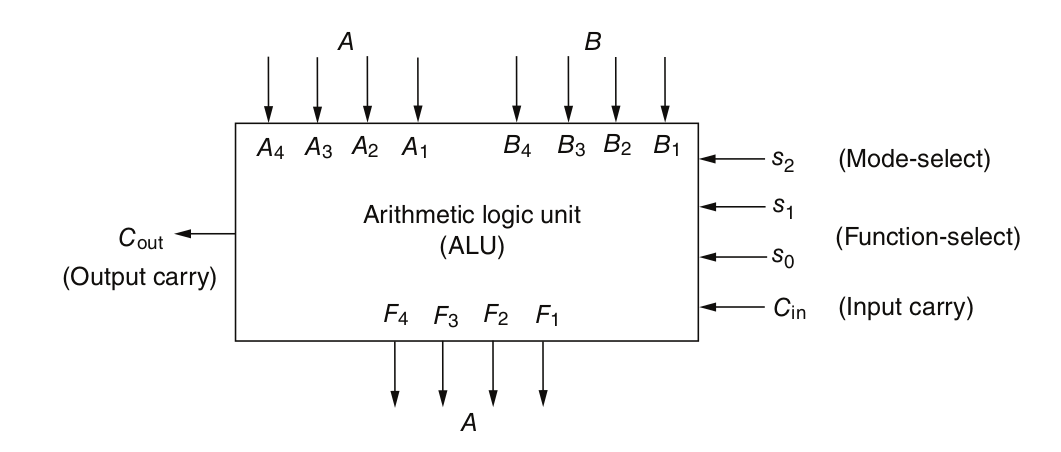
\includegraphics[width=\textwidth]{1. block diagram.png}
    \caption{Block diagram of a 4 bit ALU}
\end{figure}

\newpage
\section{Complete Circuit Diagram}

\begin{figure}[h]
    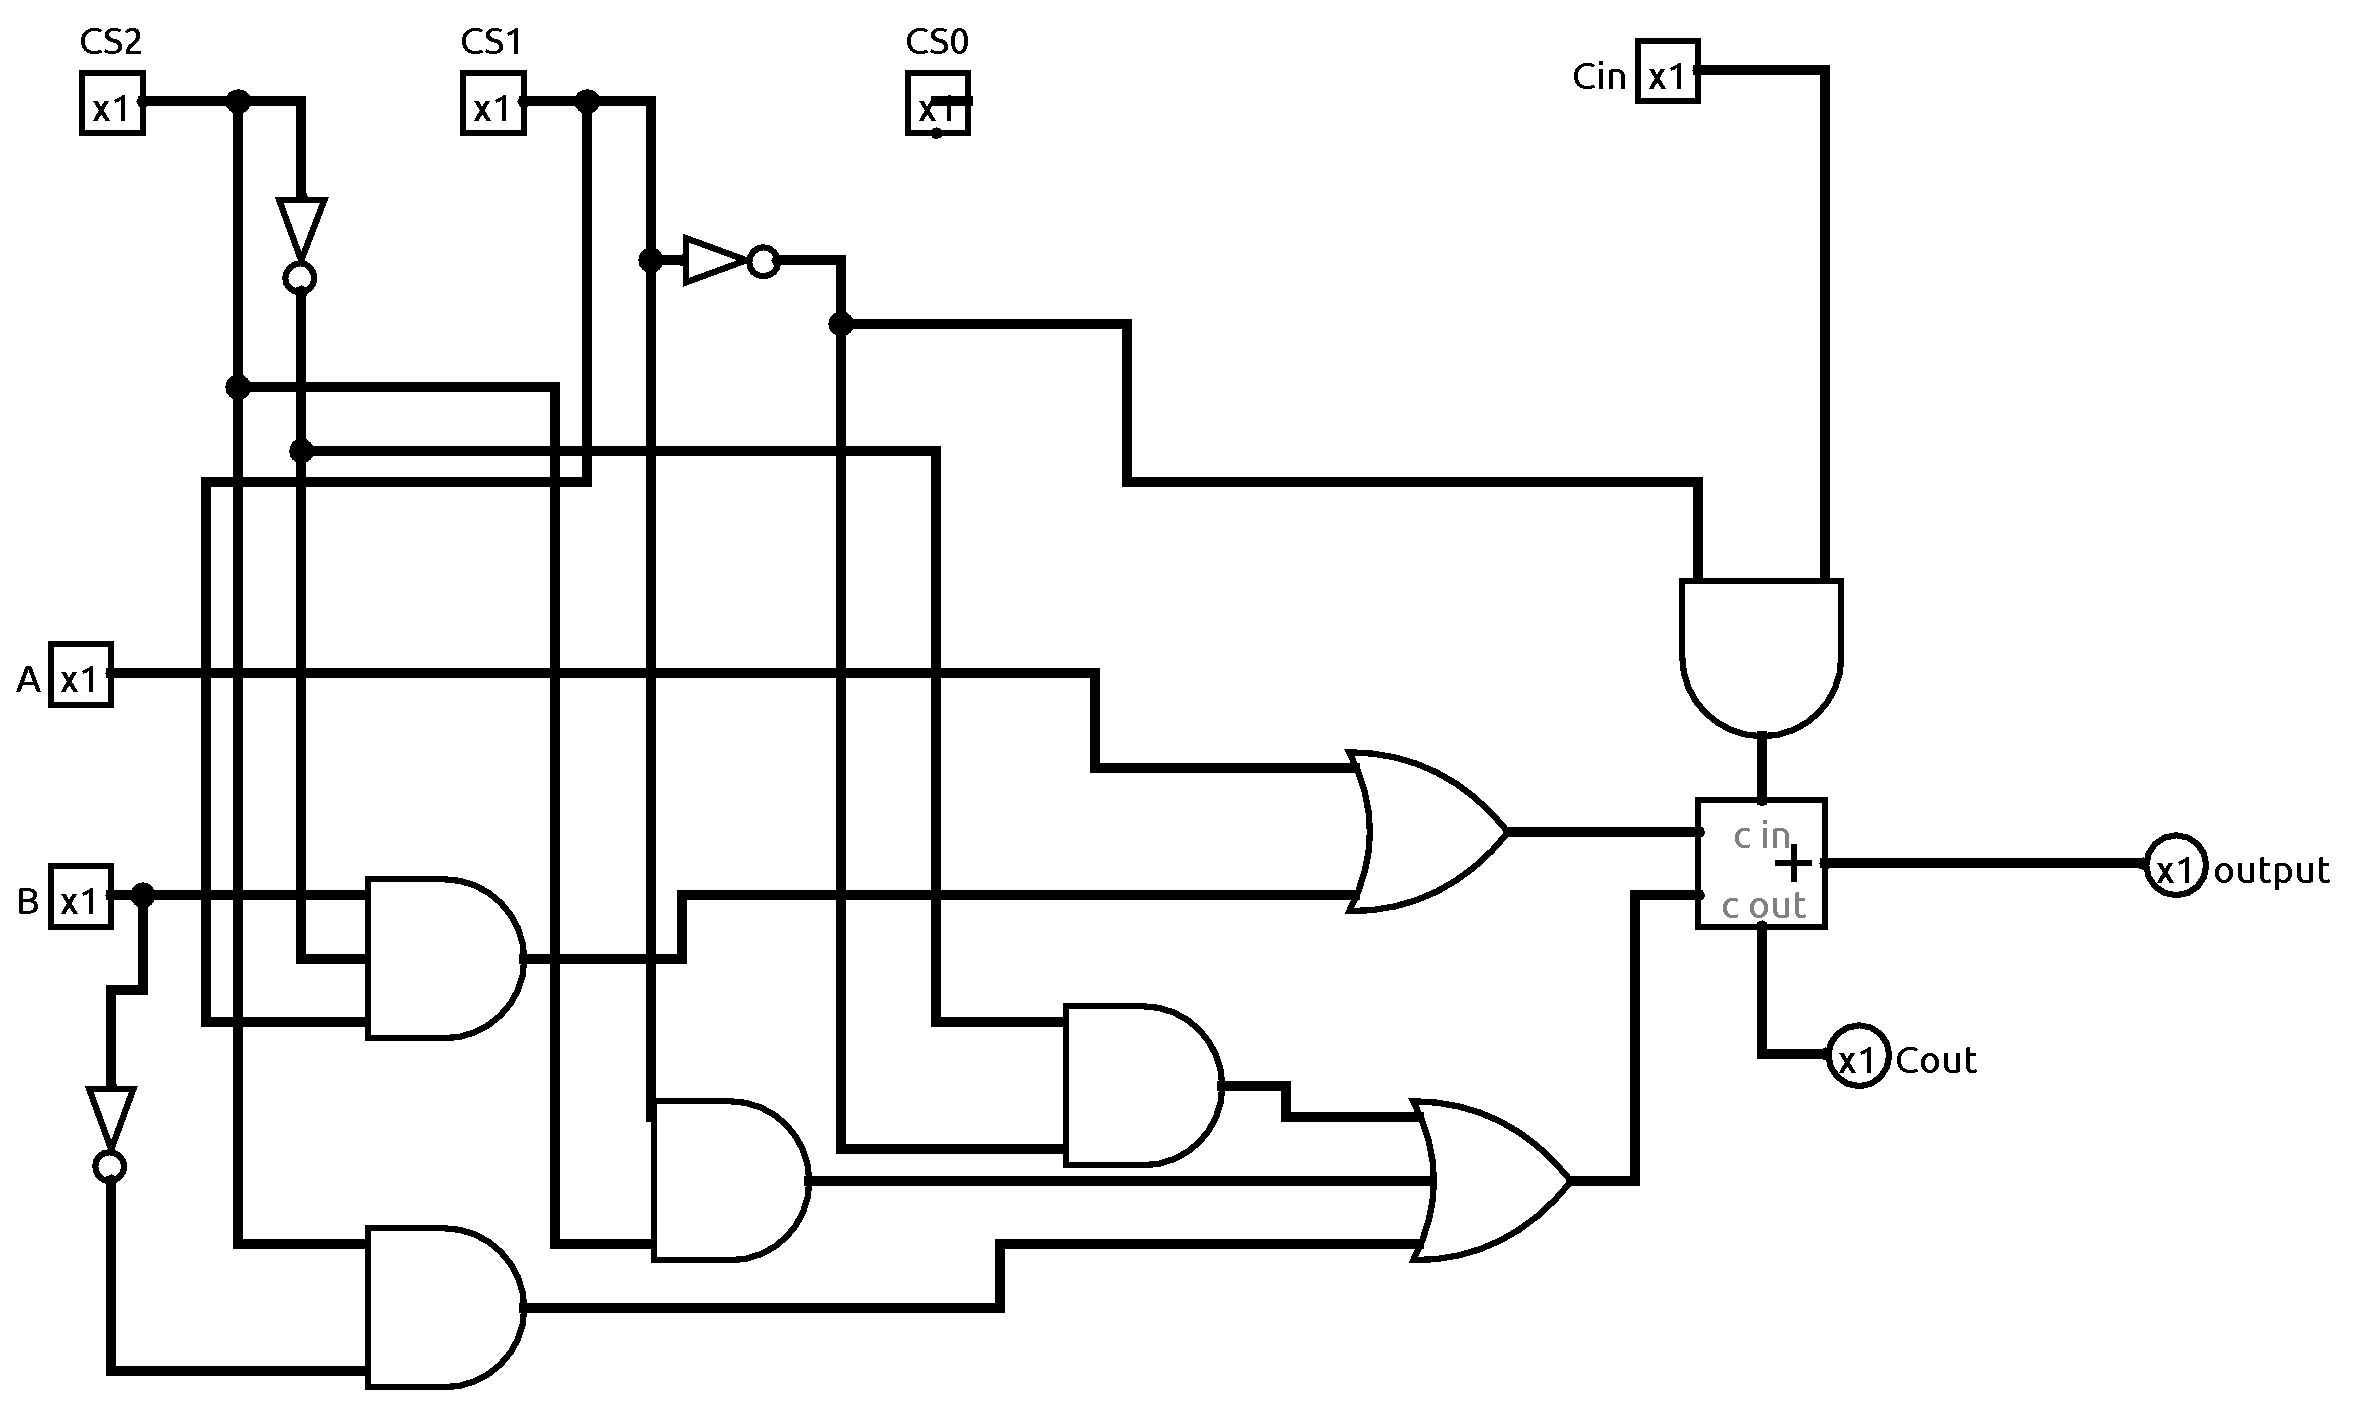
\includegraphics[width=\textwidth]{2. 1 bit alu.png}
    \caption{1 Bit ALU}
\end{figure}



\begin{figure}[!htbp]
    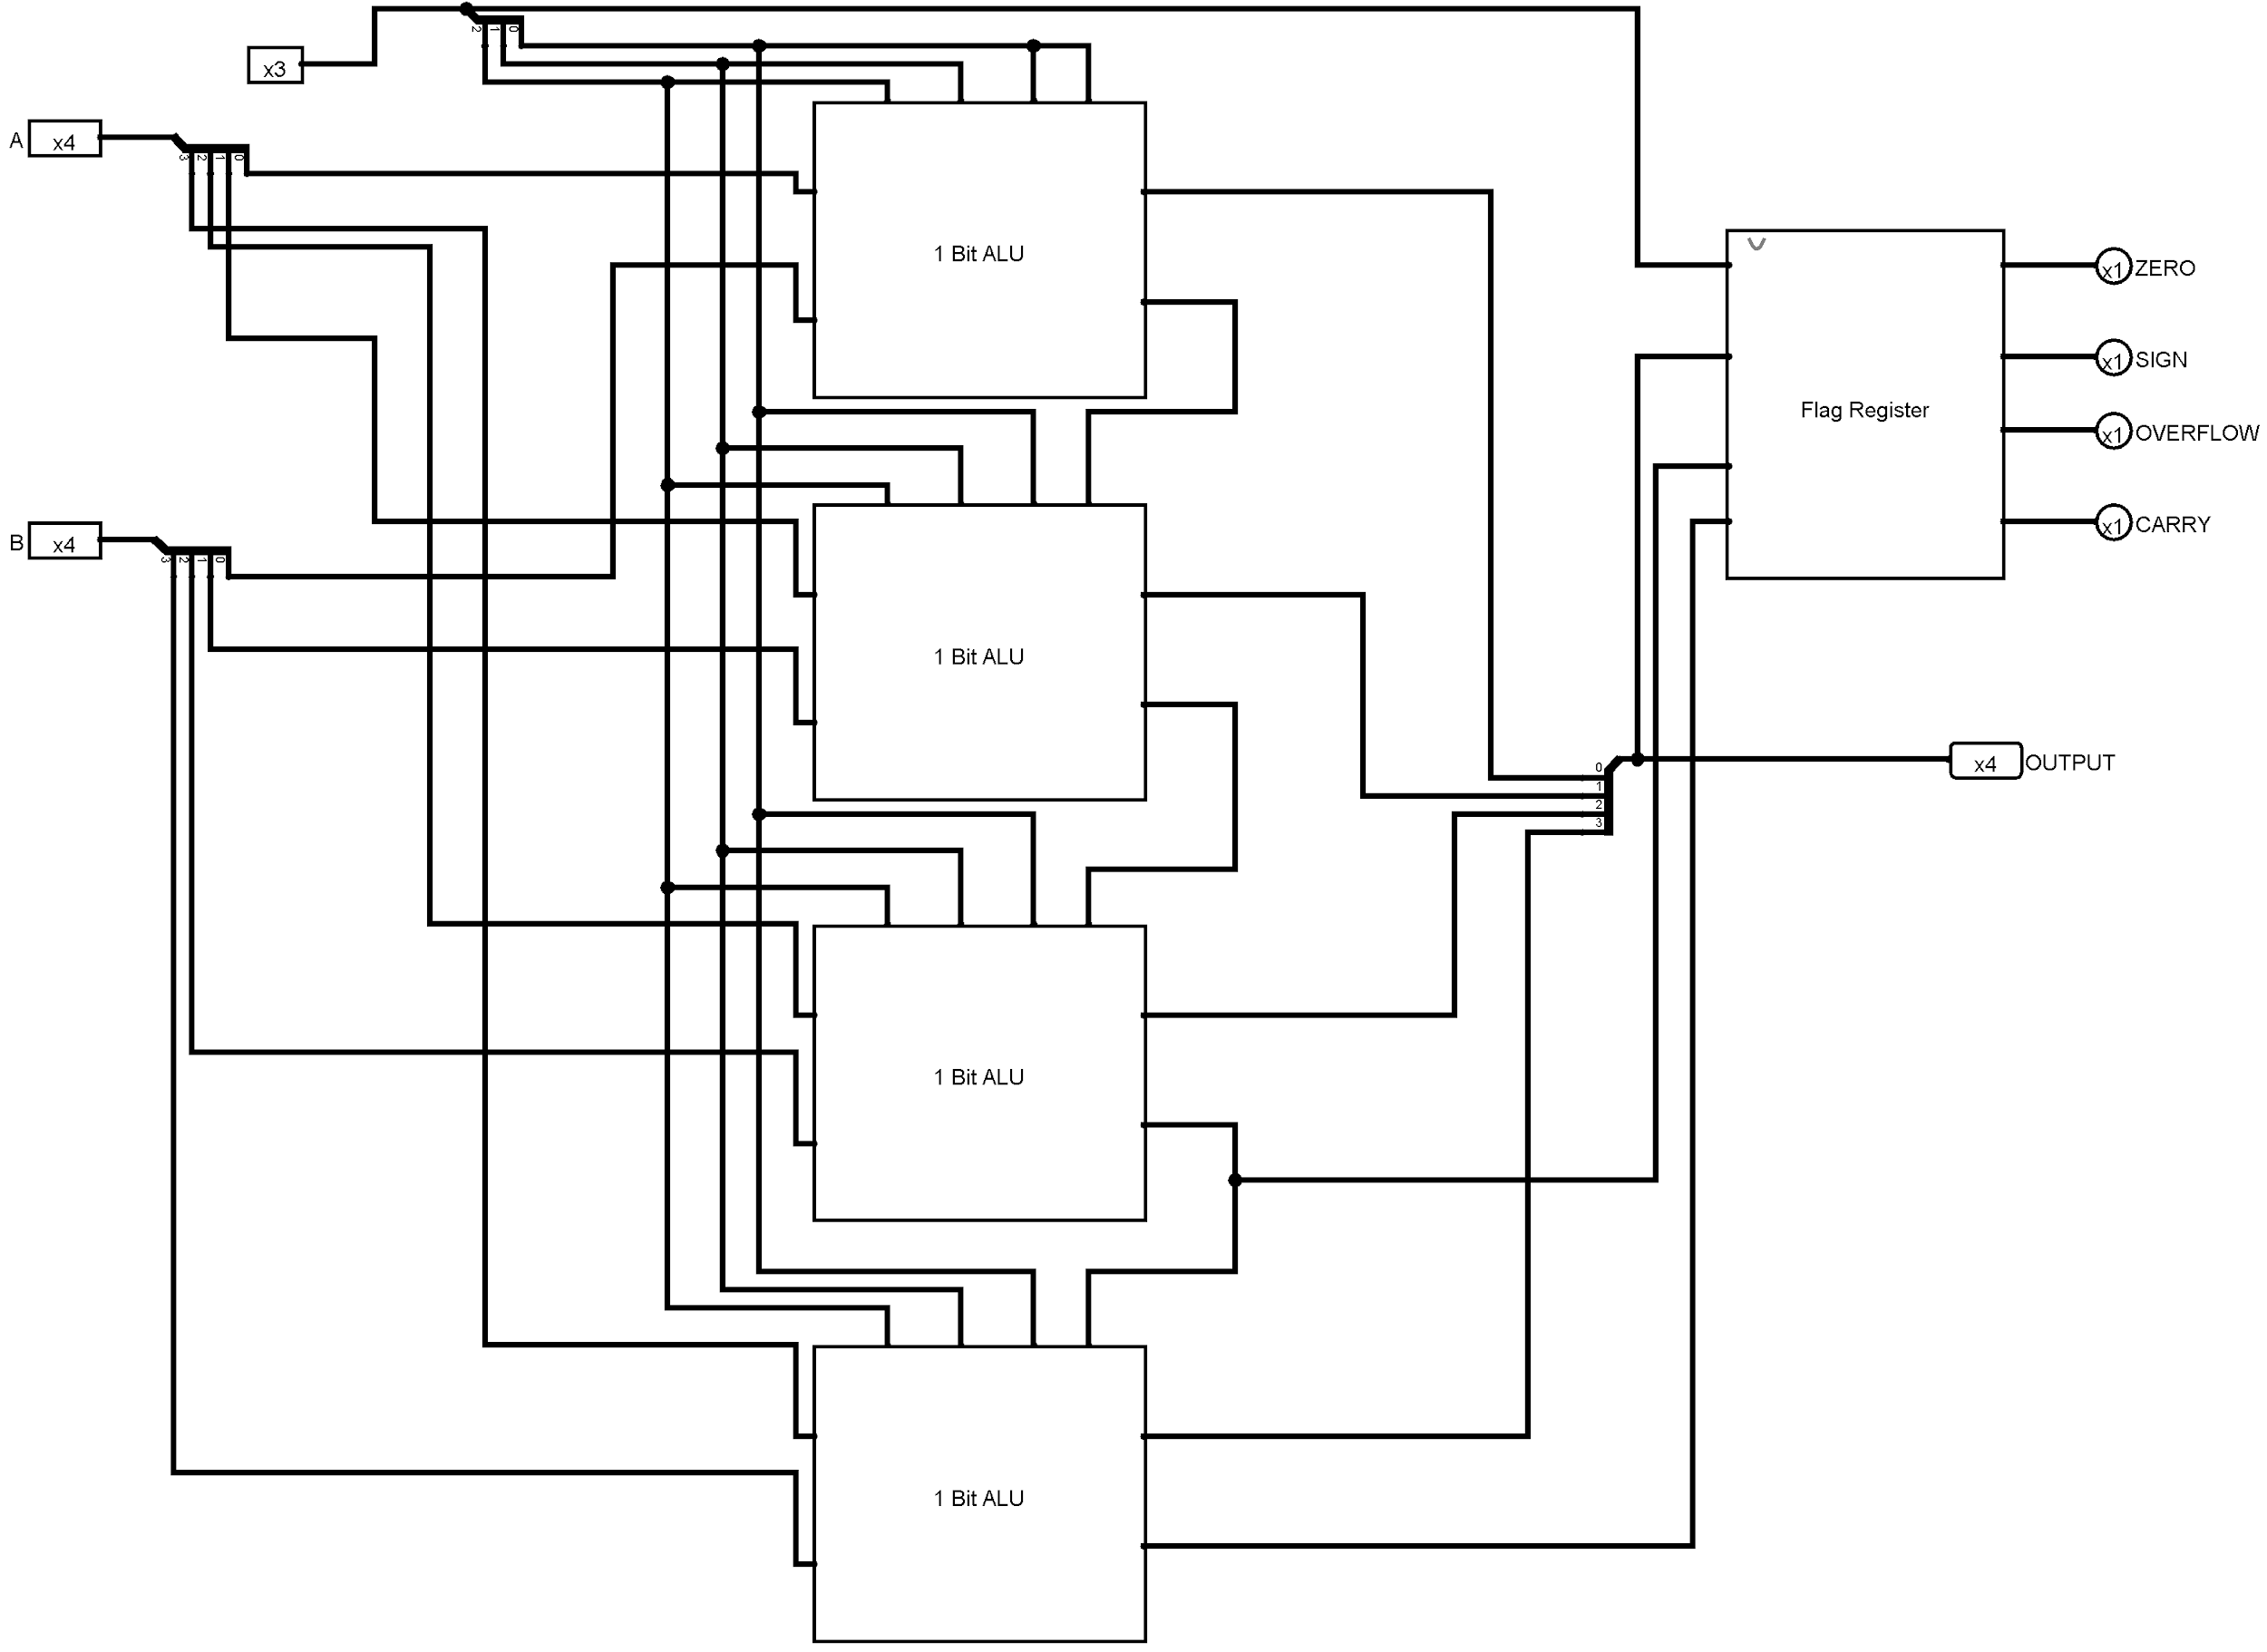
\includegraphics[width=\textwidth]{3. 4 bit alu.png}
    \caption{4 Bit ALU}
\end{figure}

\newpage

\begin{figure}[h]
    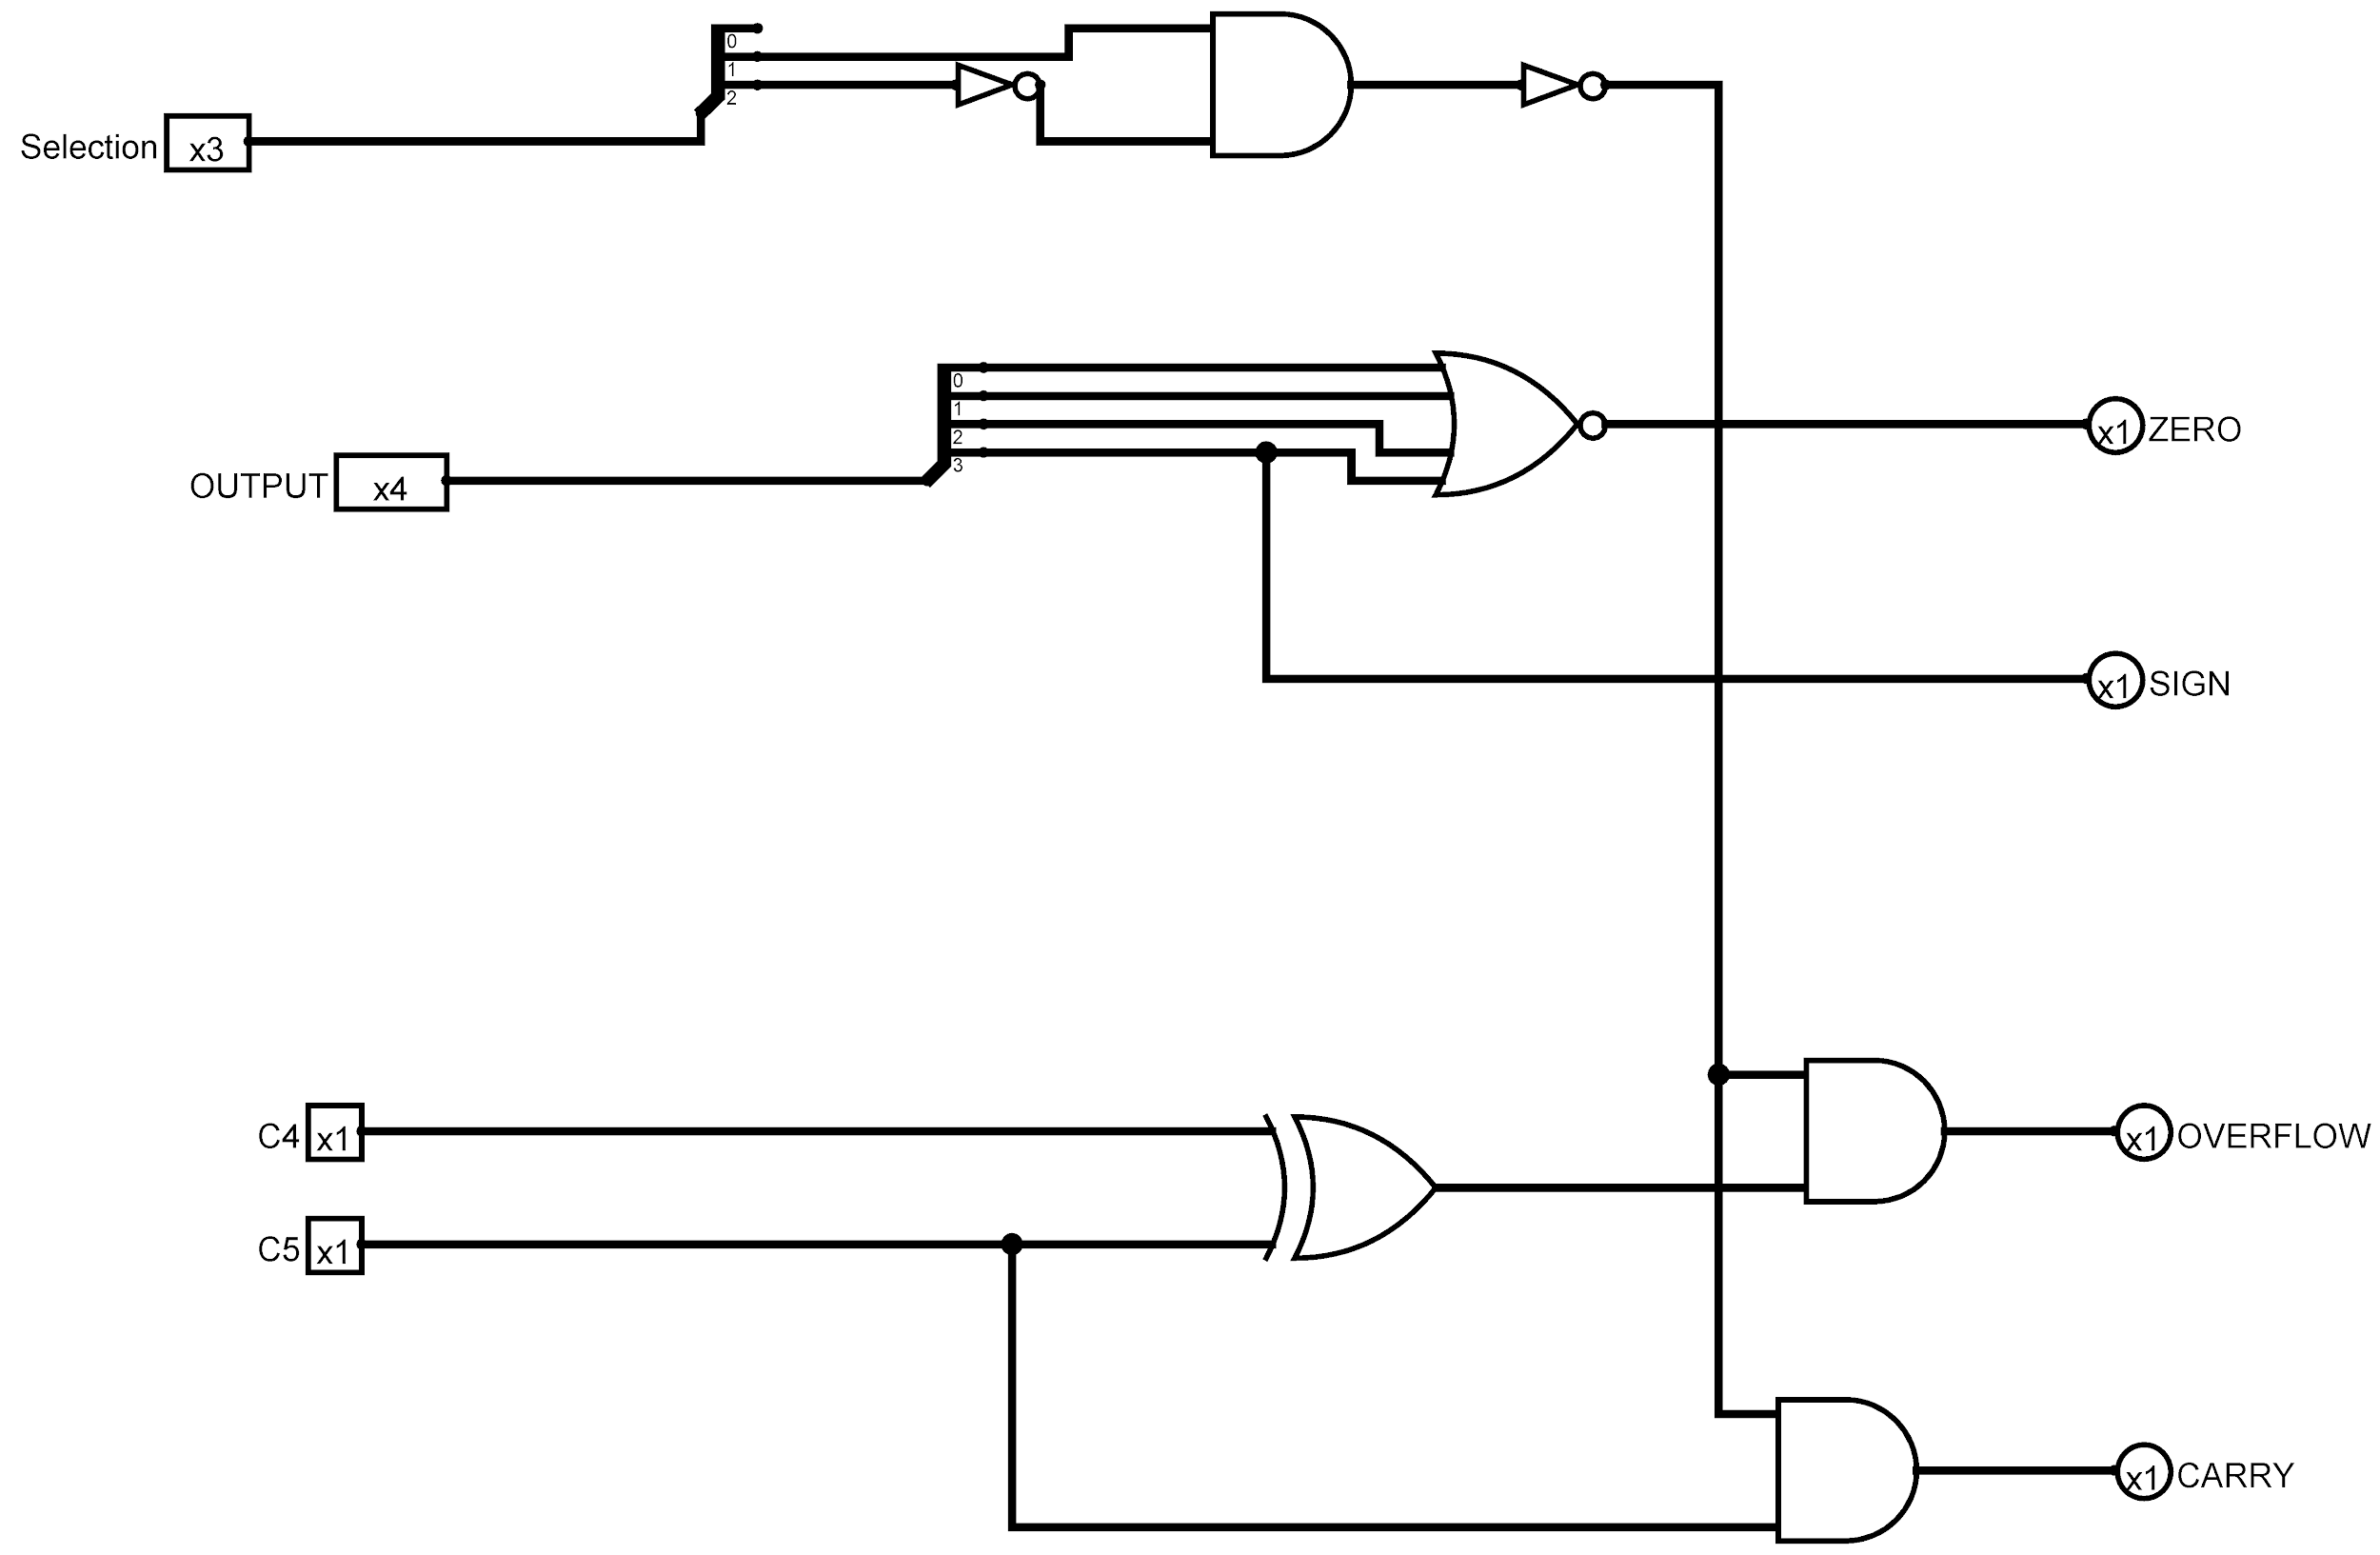
\includegraphics[width=\textwidth]{4. flag register.png}
    \caption{Flag Register}
\end{figure}

\textbf{Additional combinational circuit for the Flag Register:}
\newline
The Flag register requires the Carry flag (C) and the Overflow flag (V) to be cleared (0) after a logical OR operation. The ALU performs an OR operation when s2=0 and s1=1; Therefore,
\newline
The modified carry = $C(s_2’s_1)’$
\newline
The modified overflow = $V(s_2’s_1)’$


\section{Total Number of ICs Used in the Implementation}

\begin{table}[ht]
\centering
\begin{tabular}{|c|c|c|c|}
    \hline
    \textbf{Name} & \textbf{IC no.} & \textbf{Number of Gates} & \textbf{Number of ICs} \\
    \hline
    OR & IC 7432 & 15 & 4 \\
    \hline
    AND & IC 7408 & 27 & 7 \\
    \hline
    NOT & IC 7404 & 15 & 4 \\
    \hline
    Adder & IC 7483 & 4 & 4 \\
    \hline
\end{tabular}
\end{table}

\newpage
\section{Simulator Info}
Logisim - Java Platform (Version 2.7.1)

\section{Discussion}
\begin{itemize}
  \item We designed the ALU in Logisim simulator.
  \item Initially we designed an 1 bit ALU and from it by cascading we designed the 4 bit ALU according to the functions that were given as our task. And lastly, we designed a Flag register to show the values of C, S, Z and V flags. We combined the two circuits together and got the 4 bit ALU. 
  \item For the designing of ALU according to the given functions, we formed a truth table, used it to construct the required k-maps for $X_i$, $Y_i$ and $Z_i$, derived equations for each of them and used the equations to design the 1 bit ALU.
  \item  We used cs0 as our initial $C_{in}$ bit and the other cs1 and cs2 as selector bits for the required arithmetic and logical operations.
  \item One important thing to mention here is that the flag register in the ALU does not fully comply with the rules of assembly language in the sense that the values of C, V, S or Z bits may change after a logical NOT operation even though assembly language rules clearly dictate that NOT operations should not affect the Flag register at all.
\end{itemize}


\end{document}
